\sectionframe{Period-adding the Simplified Model}
\section{Period-adding}

\begin{frame}{Parameter Changes Needed}
	\vspace{-1em}
	\begin{figure}
		\includegraphics[width=.4 \textwidth]{60_MinimalRepr/Cobweb_E16/result.png}
		\includegraphics[width=.4 \textwidth]{62_MinimalRepr_Adding/Cob_1_ZCorn/result.png}
	\end{figure}
	\begin{itemize}
		\item We got rid of the local minimum on branches $f_\A$ and $f_\C$
	\end{itemize}
\end{frame}

\begin{frame}{Period-adding in our Model}
	\begin{figure}
		\includegraphics[width=.4 \textwidth]{62_MinimalRepr_Adding/2D_Regions_1/result.png}
		\quad
		\includegraphics[width=.4 \textwidth]{62_MinimalRepr_Adding/2D_Period_larger_adding_zoomed/result.png}
	\end{figure}
	\todo{Labels wrong}
\end{frame}

\begin{frame}{The Path to Period-adding (Schematic)}
	\begin{figure}
		\only<1>{
			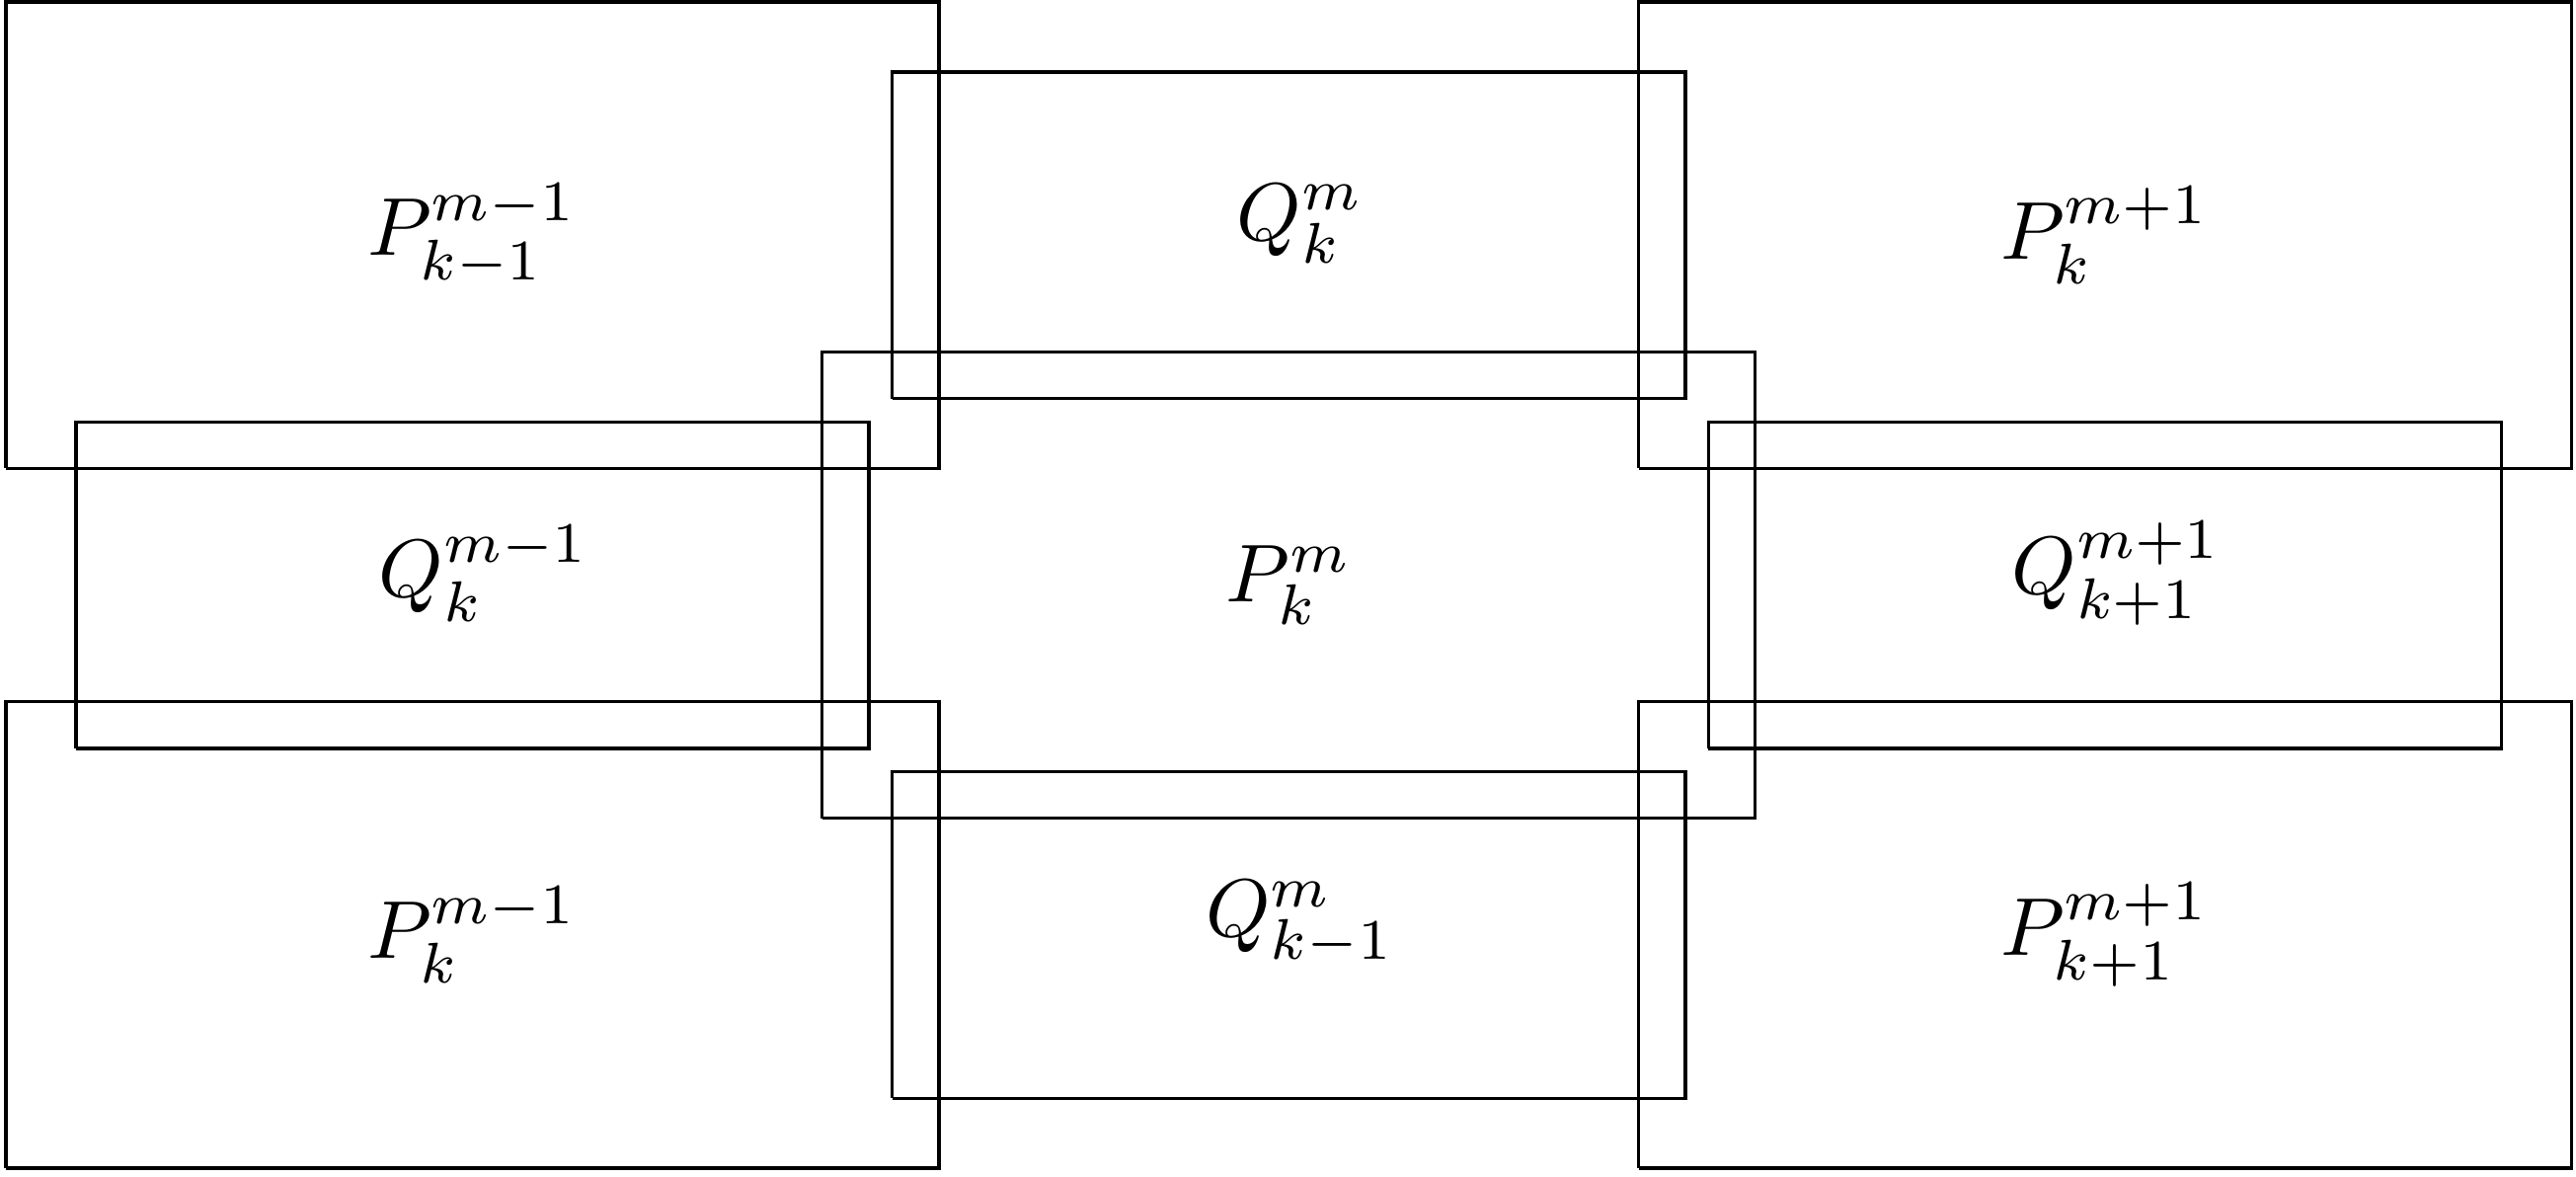
\includegraphics[width=.7 \textwidth]{../../Report/Figures/Schemas/BeforeAdding/schema.png}
			\todo{Different alignment}
			\todo{Labels wrong}
		}
		\only<2>{
			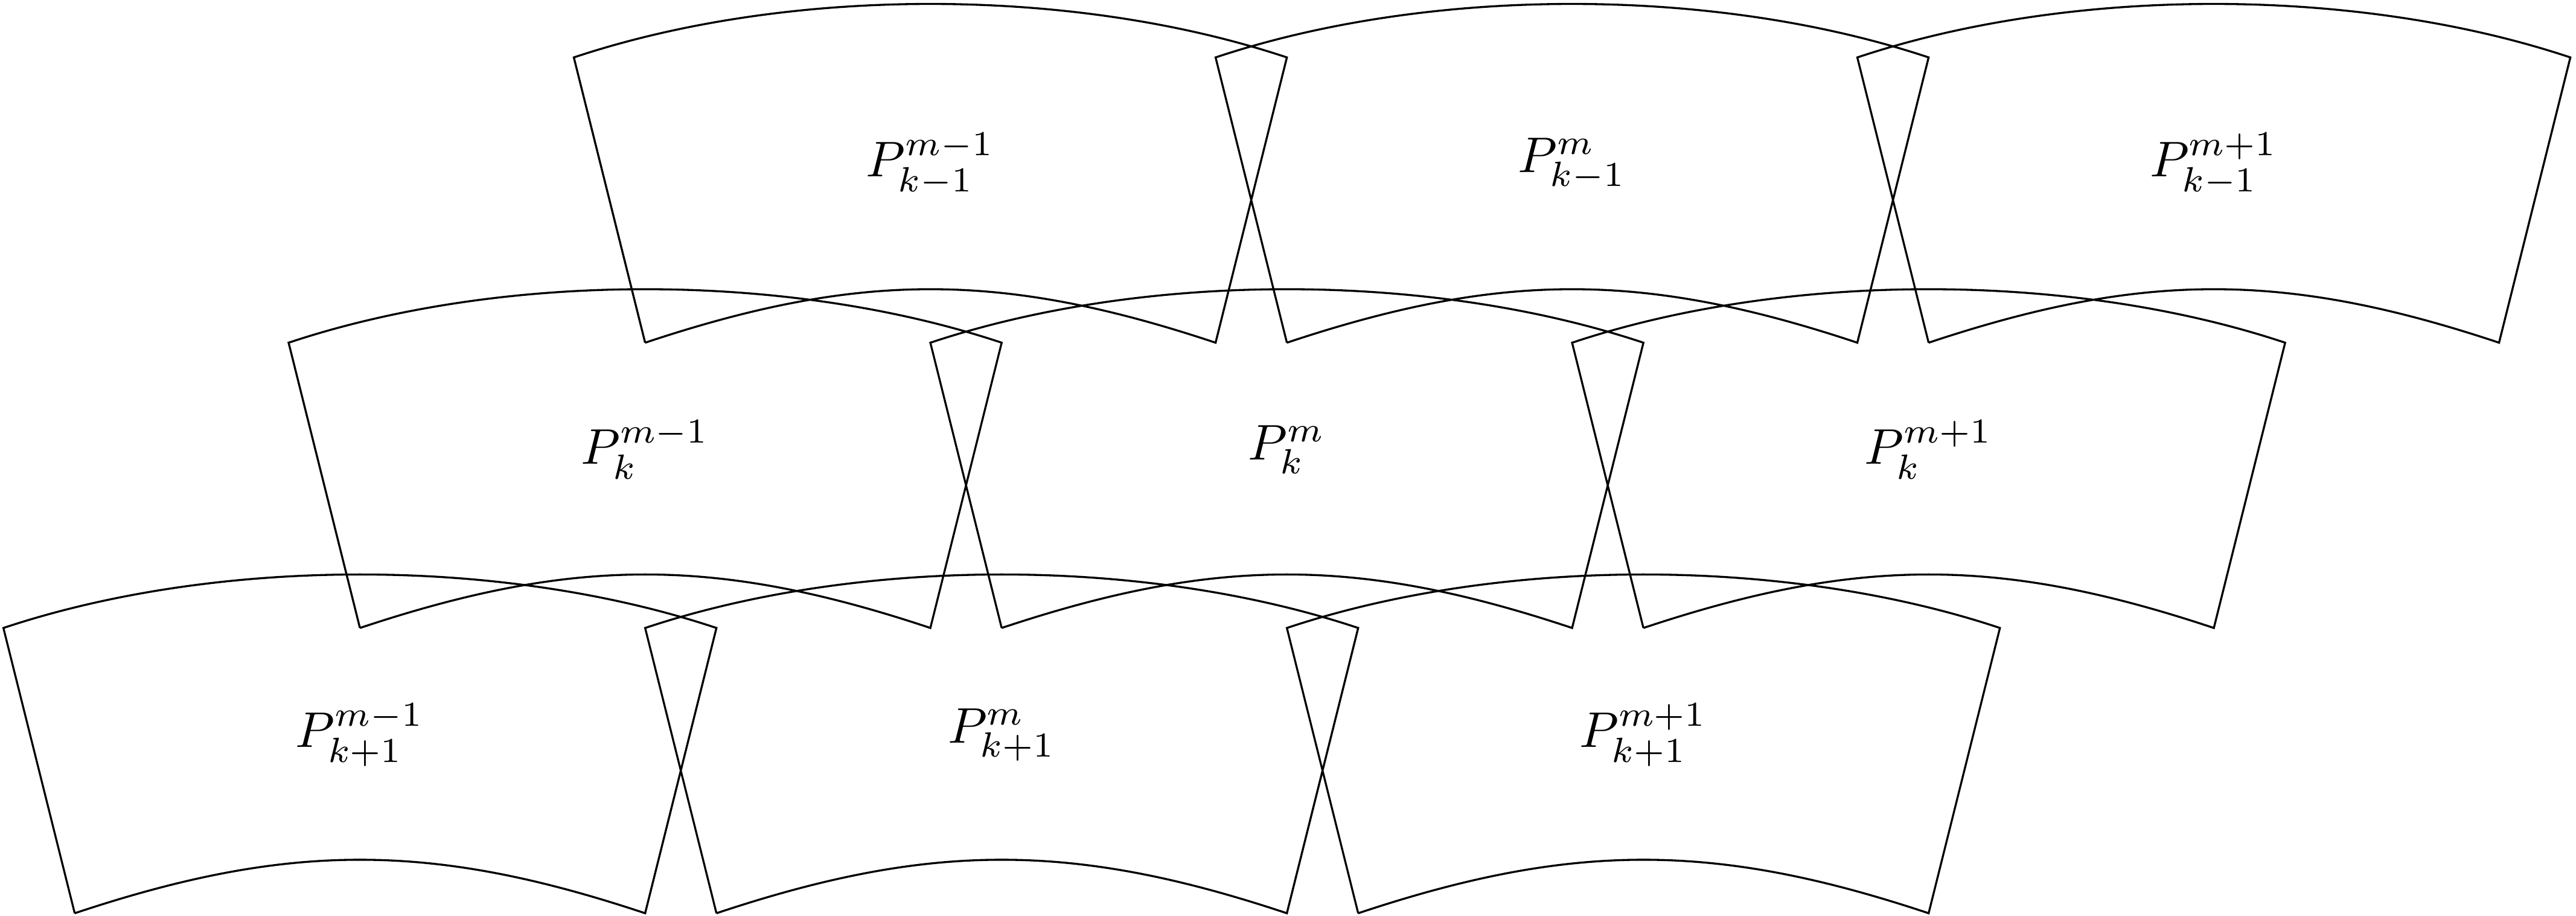
\includegraphics[width=\textwidth]{../../Report/Figures/Schemas/DuringAdding/schema.png}
			\todo{Mark Q areas, adding areas}
		}
		\only<3>{
			\todo{Final with complete adding}
		}
	\end{figure}
\end{frame}

\begin{frame}{The Path to Period-adding (Numeric)}
	\begin{figure}
		\includegraphics[width=.4 \textwidth]{62_MinimalRepr_Adding/2D_Regions_2.725/Manual/result.png}
	\end{figure}
	\todo{Labels wrong}
\end{frame}

\begin{frame}{Describing the Bifurcation Structures}
	\vspace{-1em}
	\begin{figure}
		\only<1>{
			\includegraphics[width=.4 \textwidth]{62_MinimalRepr_Adding/2D_Period_larger_adding_zoomed/result.png}
			\todo{Labels wrong}
		}
		\only<2>{
			\includegraphics[width=.4 \textwidth]{62_MinimalRepr_Adding/1D_Period_larger_adding/Manual/result.png}
			\qquad
			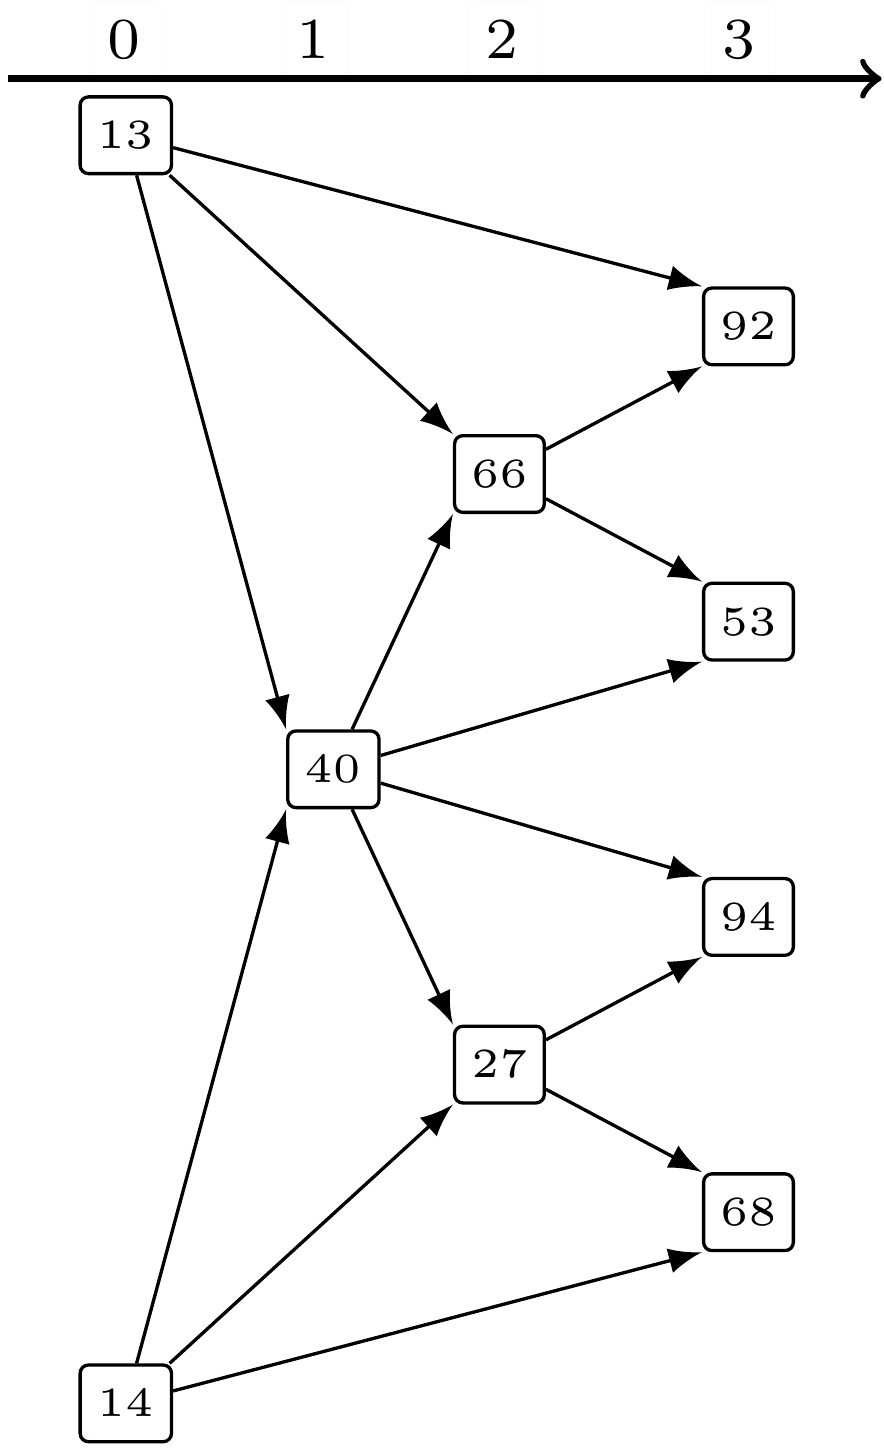
\includegraphics[width=.25 \textwidth]{../../Report/Figures/FareyTrees/Minrep_Adding_larger_Full_Period_3/adding.pdf}
		}
		\only<3>{
			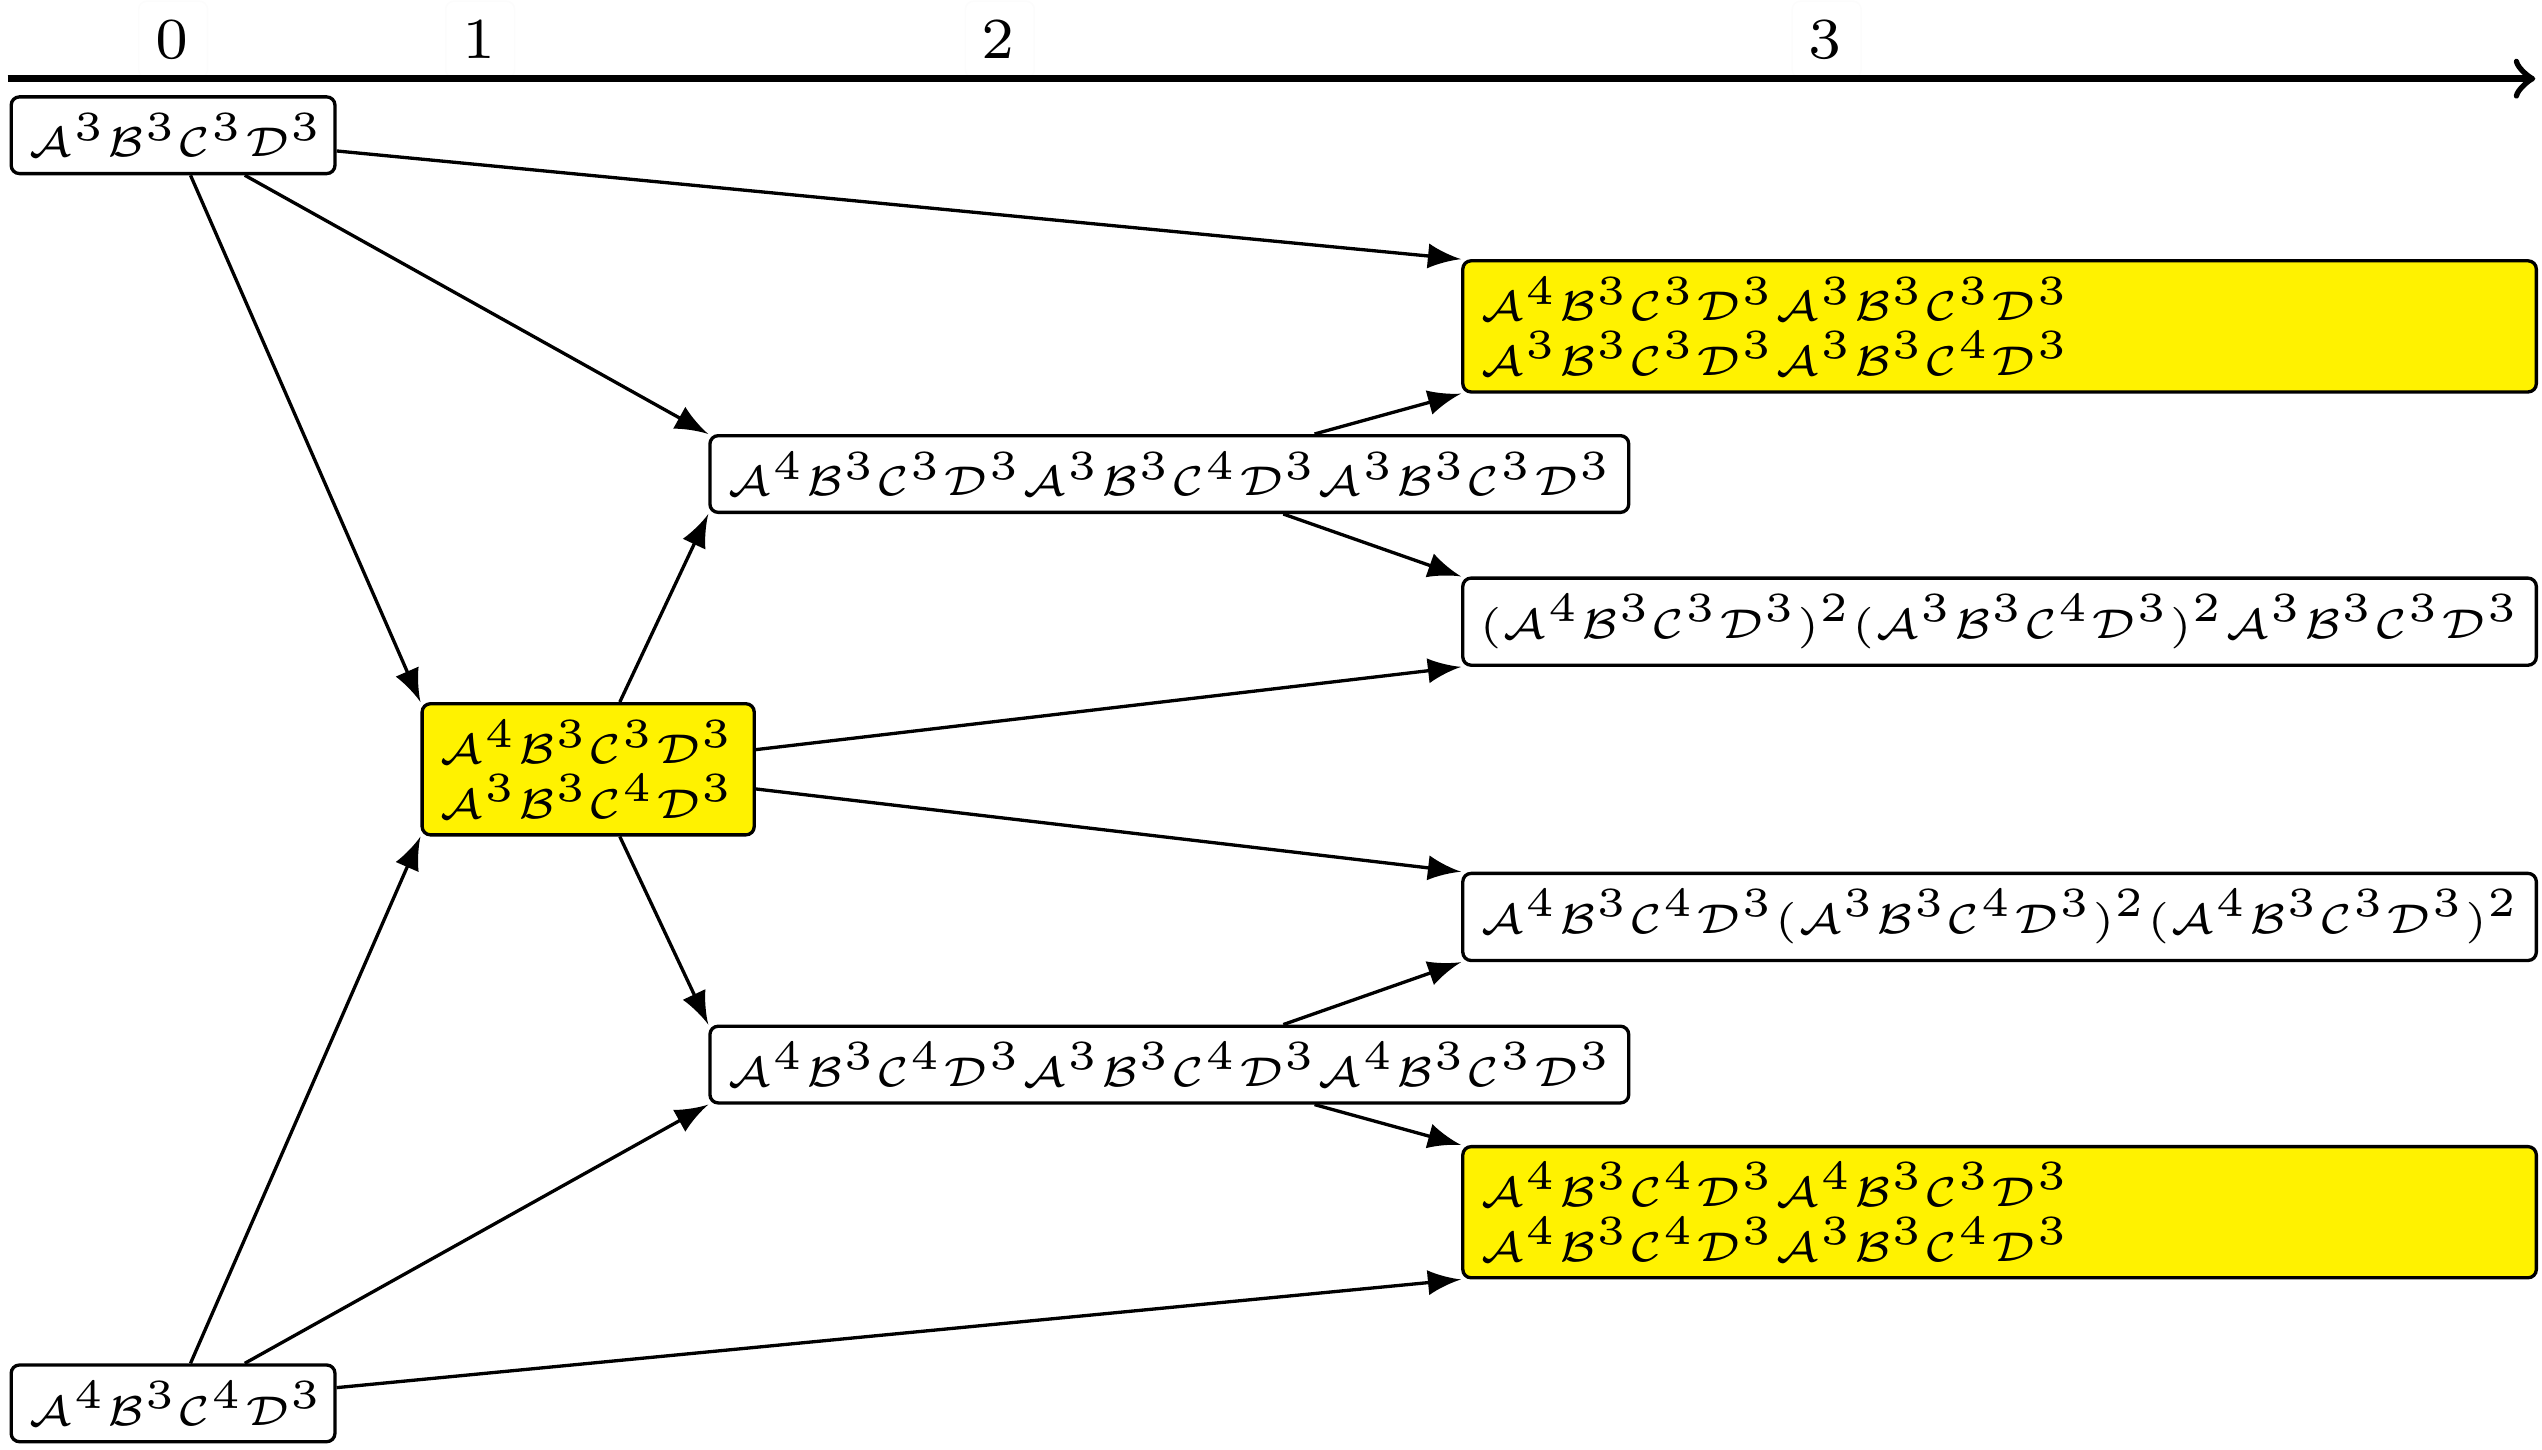
\includegraphics[width=.7 \textwidth]{../../Report/Figures/FareyTrees/Minrep_Adding_larger_Full_3/adding.pdf}
		}
	\end{figure}
\end{frame}

\begin{frame}{Problems with the Bifurcation Structures}
	This is not period-adding
	\pause
	\begin{itemize}
		\item Periods don't add \pause
		\item Cycles don't concatenate
	\end{itemize}
\end{frame}
